\documentclass[12pt, titlepage]{article}

\usepackage{float}
\usepackage{caption}
\usepackage{graphicx}
\usepackage{listings}
\usepackage{geometry}
\usepackage[T1]{fontenc}
\usepackage[american]{babel}
\usepackage{hyperref}
\usepackage{setspace}
\usepackage{verbatim}
\usepackage{fancyhdr}

\geometry{margin=1in}
\graphicspath{{EEimages/}}

\begin{document}
\doublespacing
% Title page will be in word doc

\renewcommand{\contentsname}{Table of Contents}
\pagenumbering{gobble}
\tableofcontents
\newpage
\pagenumbering{arabic}

% Headers
\renewcommand{\headrulewidth}{0pt}
\renewcommand{\footrulewidth}{0pt}
\fancyhead[R]{fwj493 \thepage}
\fancyhead[L]{}
\cfoot{} % Clear bottom page number
\pagestyle{fancy}

\noindent
\thispagestyle{empty}
\textbf{\Large Effectiveness of Various Recurrent Architectures on Music
Generation}

\section{Introduction}
As technology develops, more and more computationally expensive tasks can be
utilized. One growing field exemplifying this is the category of deep learning
algorithms, that can model very complex data.  Recurrent networks specialize in
this task, being able to model time series, such as speech. This paper will
discuss the effectiveness of using different types of deep learning algorithms
to model another type of time series, music. The model will then be utilized to
generate music, to see how well it is able to model music based on other samples
of music. The model will also be trained using unsupervised learning techniques,
to see the relative abilities of each model to remember sequences, or compress
the music.

\section{Models}
The models that will be tested and evaluated will be different variations of
state of the art recurrent neural networks, and their effectiveness will be
judged by the time they take to minimize the mean squared error of the music
file that they are trying to model.

Although the models may have different structures, in general all the listed
models, have some cost function that they are trying to minimize. Typically, and
in this paper, the cost function is assumed to be minimized with gradient
descent.  As further elaborated by Sebastian Ruder, a Ph.D student in natural
language processing, gradient descent is an algorithm in which the gradient of a
function with respect to some parameter of the function is multiplied by some
factor, and then the parameter is updated through subtracting the calculated
product of the gradient and factor~\cite{graddescent}

\subsection{Logistic Regression Model}
To understand learning algorithms, the logistic regression model is notable, as
it can be thought of a building block for larger models. As described by Andrew
Ng's online course on machine learning, logistic regression
models are classification models~\cite{ngcourse}.

This means that they are typically used to predict the probability of a
situation or event, based on data. One example used Ng's course describing these
models is the problem of determining how likely someone is to develop cancer
based on the data relating to the medical history of the patient~\cite{ngcourse}.

One method in which they could be used, as described in Ng's machine learning
course, is through first converting the existing data, such as medical records,
into a vector of numbers~\cite{ngrepr}. Then, continuing off of the description
from the course, the model multiplies a weight value to each input number, and
sums up the products of weight value with input numbers~\cite{ngrepr}. The
weight can be thought of as the significance of each input, and the sign being
whether or not the input value is positively or negatively correlated to the
data. After summing the product of weight values with input values, the sum is
passed into the sigmoid function, which changes the sum into a value between 0
and 1 as Ng describes~\cite{ngrepr}. This new value, between 0 and 1 is the
probability of an event happening, and is compared against the correct value,
being whether or not the event, such as cancer, did or did not happen based on
the data~\cite{ngrepr}.

These models, however, have limitations as to how complex the data in which they
can model. For example, as they are classification models, they are not very
applicable for the task of music generation, which requires predicting integer
values, as opposed to true or false labels.

\subsection{Neural Networks}
To understand the other models, one must first understand what a neural network
is. As explained in Michael Nielsen's online book, neural networks are a type of
model, that attempts to try to learn patterns within data through a method of
modeling neurons in the brain with sigmoid functions~\cite{nielbook}. A logistic
regression model predicts a value between 0 and 1 given some data as previously
mentioned~\cite{ngrepr}. To stack logistic regression classifiers means to put
the output of one set of classifiers as the input as the next set of
classifiers. Through this, a neural network is created. As implied by Nielsen's
description of neural networks in his book, the neural network was inspired by
biological systems, since the outputs of each classifier can be thought of as
activations for synapses in a brain~\cite{nielbook}. Because neural network
models have more weights and layers than logistic regression classifiers,
intuitively it seems that neural networks are more powerful in what types of
data they can represent. Thus, as music is complex, a more powerful model should
be used.


%\subsection{Deep Learning}
%Deep learning in this paper will be interpreted as is interpreted in LeCun et
%al.'s presentation: any model with ``multiple levels of
%abstraction''~\cite{dlppt}.

%Deep learning algorithms are capable of complex tasks, potentially due to their
%increased size. For example, one applications of these deep networks is
%SyntaxNet, an algorithm that can correctly determine the grammatical structure
%of a sentence, such as determining what the direct object of a sentence
%is~\cite{syntaxnet}. Because of these successes with deep architectures, they
%will be tested to see if they are powerful enough to generate music, as they are
%very powerful in other areas.


\subsection{Vanilla Recurrent Neural Networks}
According to Orr's class website at Willamette University, recurrent networks
are a variation of neural networks that can model time series data, which is as
a result, can be used in natural language processing tasks~\cite{rnnintro}. As
Orr elaborates, vanilla recurrent neural networks accomplish this task through
being a neural network, except with some connections going through
time~\cite{rnnintro}. In this paper, the activation of a hidden node can be considered as
$$a_t = W\cdot a_{t-1} + W\cdot I_t + b_a$$
where $a_t$ is the activation at time t, W is the corresponding weight matrix,
$a_{t-1}$ is the activation of the node at one time step earlier, and $I_t$ is
the input at that time. The activation goes through a nonlinearity, such as a
sigmoid function before being passed to the next node~\cite{rnnintro}. These
models theoretically can model time series, and some examples given by Orr's
class are speech recognition and learning the grammar of languages, but in
practice they do not have much memory, as compared to other models, such as
LSTM's~\cite{rnnintro}\cite{lstm}. As the length of the time series increases,
these models become prone to ``forgetting'' earlier samples in the input data,
as demonstrated by Horchreiter 's paper, as recurrent nets were outperformed on
tasks requiring long term memory by LSTM's~\cite{lstm}. Thus, other more
complicated models should probably be used for the task of music generation, as
intuitively, music seems to have long term dependencies.


\subsection{Long Short Term Memory Networks}
A model that, developed by researches in the Technical Institute of Berlin,
attempts to overcome the short term memory of vanilla neural networks and solve
the vanishing gradient problem is the long short term memory
network~\cite{lstm}. As described in Horchreiter's paper, these networks,
through using cells and vectors that can be modified by the network, can store
long term information~\cite{lstm}. They do this through generating ``memories'',
through the function:
$$M = \tanh(W\cdot C + W\cdot I_t + b_M)$$
where C denotes the cell state of the network, as originally envisioned by
Horchreiter~\cite{lstm}. However, these networks are more computationally
expensive, due to the significantly increased complexity of the model, as the
model has more weights and calculations required involving the memory cell, as
found in my experiments. As a result, tasks such as computing the gradient, the
error, or predicting something with these models takes more time than a
traditional recurrent neural network, as the LSTM model took significantly
longer on those tasks than the traditional networks.

However, the accuracy of the LSTM can be improved if it is allowed to reset it's
memory state. As originally suggested by Gers, if a LSTM's memory is multiplied
by a ``forget gate'', which is a value between 0 and 1, the LSTM can predict
even longer sequences~\cite{forgetgate}. Through forget gates, the memory of
LSTM's are restrained from growing too large, which would cause the memory cells
to be useless~\cite{forgetgate}. Also, this addition of a forget gate
intuitively, as useless memory should be discarded. In practice, what this might
mean for music generation is that the theme of a song may completely shift, as
the LSTM could have ``forgotten'' the structure of the song earlier. The LSTM's
in this paper will be assumed to have forget gates.

The LSTM accuracy can also be further improved through adding ``peephole
connections''~\cite{lstmpeep}. These are simply a connection between the memory
cell of the LSTM to the forget gates and remember gates. According to Gers'
paper, through these peep hole connections, the LSTM can model short term
changes and fluctuations more accurately~\cite{lstmpeep}.

During training of LSTM's, a notable technique that will be used it large
initialization of the forget gate bias, which if not proper initialized, will
cause problems with the gradient flow of the LSTM~\cite{lstmbias}. Through
initializing a large forget gate, Jozefowicz and others have demonstrated that
this enables LSTM's to learn long term dependencies better, which will also be
used within this paper~\cite{lstmbias}. In this manner, the LSTM mentioned in
this paper will be trained faster.


\subsection{Gated Recurrent Units}
Another variation off of recurrent networks are gated recurrent units, which
follow a similar approach to LSTMs. As defined in Cho et al., instead of
completely reassigning the models hidden state each timestep, it instead updates
its hidden state through the equation:
$$h_t = (1 - z) * h_t + h'_t $$
z is a unit that the model calculates, and is bounded between 0 and 1 with the
sigmoid activation function~\cite{gru}. As a result, this type of network also
has been found to have long term memories, and has been found to be comparable
to the performance of LSTM's according to the researchers at the University of
Montreal~\cite{gru}. These models also seem to be faster to compute than LSTM's,
perhaps due to their lower number of weights in my implementation. Thus, this
model will also be tested against LSTM's in its performance.


\subsection{Clockwork Recurrent Neural Network}
Another attempt to increase the memory of a vanilla recurrent neural network, is
the clockwork recurrent neural network. Originally developed by Koutnik and his
colleagues, these networks are identical to vanilla networks, except their
hidden layer is partitioned~\cite{cw-rnn}. Each partition of hidden units is
calculated for only some of the input, and thus is not updated at every time
step~\cite{cw-rnn}. As a result, the partitions that are updated less often
serve the purpose of being the memory for the network, and enable the model to
``remember'' better than normal recurrent networks~\cite{cw-rnn}. Also, these
networks are less computationally expensive than long short term memory
networks, resulting in faster compile and training times~\cite{cw-rnn}. In its
original paper, it was concluded that it has significantly more representational
power than LSTM's and GRU's with the same number of parameters, suggesting that
this network is the most efficient network of them all~\cite{cw-rnn}.

%\subsection{Restricted Boltzmann Machines}
%The restricted Boltzmann machine is an unsupervised learning algorithm that
%attempts to determine the distribution of a sample of input using an energy
%based model. This means that the model finds a way to map an ``energy'' to each
%input, and then probabilistically finds the lowest energy input. This is useful,
%as the model can be trained to associate known input data with lower energy, and
%randomly generated data with higher energy. Since this model generates hidden
%units to determine the energy of the system, the hidden units can be used as an
%input to another model. Typically, the hidden units of a restricted Boltzmann
%machine represent some higher level relationship within the data, for example,
%the edges of a picture, perhaps. Thus, they can be used to reduce the size of
%the input by a significant amount, and speed up the rest of training. Also,
%after learning the weights for the restricted boltzmann machine, it is typically
%used as a layer for the neural network, which typically speed up training.
%However, restricted boltzmann machines are falling out of favor nowadays due to
%other initialization techniques for neural networks, and other new activation
%functions.

%\subsection{Convolution Neural Network}
%Convolutional networks are simply an element of a neural network, in which a
%filter is applied to all the elements in the input, in some pattern. Typically,
%this filter is a n by n matrix, that applied onto an image through multiplying
%each pixel value with the corresponding filter value.

%Convolution neural networks are typically used for computer vision technologies,
%as elements in an image are generally more related to each other if they are
%closer to each other. However, convolutional networks can also be used in time
%series analysis, as demonstrated by the research done by
%Abdel-Hamid~\cite{convrnn}.

%Furthermore, the startup company bought by Google, known as Deep Mind,
%successfully utilized the idea of convolutional networks to model music and
%speech, which demonstrates the potential power of convolutional nets. Their
%model, known as WaveNet, uses a neural network with no fully connected layers,
%to predict the part of a piece of music or any piece of audio~\cite{wavenet}


%\subsection{Autoencoder}
%Autoencoders are also a form of unsupervised learning algorithm, as they simply
%find a relationship within the data. They are useful as they can reduce the
%dimensionality of the data, making the computations faster for the recurrent
%neural network. An autoencoder is a two layer neural network, with the input
%layer and desired output both being a sample from the input data. The weights
%connecting the input to the hidden layer is generally referred to as the encoder
%, and the weights connecting the hidden layer to the output layer is referred to
%as the decoder. The hidden layer of the autoencoder is typically passed to more
%unsupervised learning algorithms, or the primary model that is to be used.

%The type of autoencoder used in this project will have sigmoid activation
%functions, and be trained against mean squared error. The decoder part of the
%model will utilize the identity for the activation function, being that no
%nonlinearity will be applied to the activations.

\section{Training Techniques}
Because of the aforementioned gradient problems, normal methods of minimizing
the error of these models are extremely slow. Thus, new techniques will be
investigated, although they will not all be tested.

%\subsection{Xavier Initialization}
%One method to alleviate the vanishing gradient problem is better weight
%initialization. As Glorot and Bengio found, the initialization of the weights
%affects the propagation of the gradient through the model~\cite{xavier}.
%Generally, poor initialization of neural networks in general causes the gradient
%to not be propagated as well through the network, and since the network is
%trained based on the gradients, the network will have slower convergence times
%with poor initialization~\cite{xavier}. However, with xavier initialization,
%these problems with gradient propagation are remedied, and networks
%theoretically train more quickly~\cite{xavier}

\subsection{Rprop Trainer}
The initial training method that was considered was RPROP, originally devised by
Reidmiller and Braun~\cite{rprop}. This training method utilizes only the sign
of the gradient, and has a stored matrix representing the magnitude in which the
algorithm will update the parameters~\cite{rprop}. The reason this method will
be considered is because this algorithm is not affected by the vanishing
gradient problem, or the exploding gradient problem, as the algorithm is only
dependent on the sign of the gradient, not the magnitude of the gradient, which
may be unreasonably large or small~\cite{rprop}.
Furthermore, the algorithm approaches the minimum for the error function
exponentially, as it will increase the magnitude of the update if the previous
update was in the same direction as the current update. For example, if the
first update added 1 to a parameter, and the second gradient was also positive,
the second update would add 1 multiplied with some constant, being 1.2 in this
case. As a result, the updates can potentially increase exponentially, and will
find the gradient with less iterations.

However, after implementing, it was discovered that because this algorithm can
only be used for batch learning, it is significantly slower, as the entire
training dataset must be loaded before the network can update any weights. Also,
because the computer used does not have unlimited memory, it can only handle
mini batch learning algorithms that do not require training on the entire data
set at once anyways.  As a result, this training method will not be used in this
paper, although it seemed to works for smaller models.

\subsection{RMS Prop}
A technique that was developed by Geoffrey Hinton, considered by some to be the
father of machine learning, this technique is a modification to the standard
gradient descent method that in addition, keeps a moving average of the
gradients squared~\cite{rmsprop}. Unlike gradient descent, instead of updating
each weight through its gradient, it divides the calculated gradient by the
average square root of the sum of previous gradients squared~\cite{rmsprop}. As
a result, if a weight constantly receives large gradients, the update will be
divided by a larger value, resulting in the gradient update not being too large.
Similarly, if a gradient for a weight is extremely small, the gradient will be
divided by a smaller average gradient value, resulting in a larger update for
the weights. Thus, the vanishing and exploding gradient problem can be remedied
to a certain extent through this update mechanism, and furthermore, this
mechanism can be used for mini batch learning as well as batch learning. Because
of how powerful this method is, it will be used in the experiments.

\subsection{Back Propagation Through Time}
The gradient for a recurrent neural network differs significantly from a neural
network, in that the gradient is dependent on all the data given to the network
before it, whereas the gradient for a neural network given a data sample, is
dependent only on that data sample. This process of finding the gradient
throughout the previous data samples was developed by Werbos, and is known as
back propagation through time, as to find the gradient, one needs to back
propagate through the previous data samples, which are assumed to have occurred
earlier in time~\cite{bptt}. However, if the data sequence passed to a recurrent
neural network is too long, then training the model will take a large amount of
time. Since it was found that the sample of music, being around 3 min long,
takes up significant amounts of memory and time to calculate the
gradient of with respect to the network with back propagation through time,
back propagation through time was considered as a solution that would take too
long.

However, as described in Jaeger's summary of training recurrent networks, a
modification to this algorithm can be made to speed up the training, through
learning parts of the data sequence at a time~\cite{rnntrain}. Then, instead of
calculating the gradient with respect to all of the data samples, the gradient
with respect to only the last, perhaps, 200 data samples can be utilized as an
approximation of the gradient, which is significantly faster. However, as a
result, the model may not be able to learn long term patterns within the data,
due to the gradient not being calculated with respect to all data samples.


%\subsection{Real Time Recurrent Learning}
%Although back propagation through time is simple to implement, it can be
%expensive to calculate, as it requires a complete sequence of data, to fully
%learn the data. However, another derivation of the derivative of the cost
%function gives real time recurrent learning, which is only dependent on some
%stored variables, and one data sample.  However, this algorithm requires storage
%of all of the gradients of each weight to each hidden unit. As a result, as
%large recurrent networks easily have large numbers of hidden units and weights,
%this algorithm increases the computational requirements of the recurrent network
%drastically. Furthermore, each learning step takes the order of O((hidden
%units)$^4$), according to Jaeger's calculatoins, resulting in very slow gradient
%updates for recurrent networks of moderate or larger size~\cite{rnntrain}. Thus,
%this method will not be utilized either.


\section{Comparison}
Thus, this paper will compare the effectiveness of the various models, being
LSTMs, Vanilla Recurrent Networks, and Clockwork Recurrent Neural Networks. The
error rates of each model, and the time they take to train on 5 epochs of the
training song will be used to judge their effectiveness of music generation.


\section{Implementational Details}
Python and Theano are used to test these models. Python is a programming
language, and Theano is a library for python~\cite{theano}. Theano is considered
to be fast amongst the machine learning community, which is why it is used.
Also, a gpu will be utilized to increase the performance of all models. The
music utilized for the model will have come from Youtube. Also, as it was found
that generally electronic music yielded better results, electronic Youtube music
is used for aesthetic purposes, and to get better errors to compare.
Furthermore, to aid the model, the music will be put through a Fourier transform
before having the model learn it. This is purely to produce nicer results, as
when testing without the Fourier transform, the model took longer to train and
produced more static, as opposed to the model trained on the Fourier transform.

The comparisons will be done with networks all having cell sizes, or memory
sizes, or 2048, and with input sizes of 2048. This is because it was observed
that with larger input sizes, the network learned the music better. Also, the
cell sizes of each of the respective networks were kept constant, as I thought
the cell sizes would directly impact the effectiveness of the network, and since
I wanted to compare the network structure, and not the effect of cell size, I
kept the cell sizes of all the networks constant.

However, this does not necessarily alleviate the problem as some networks may
just naturally use their memory cells more effectively than others, because of
more weight matrices. However, I did not have enough resources to test the
relationship between the number of weights and modeling capability of the
network.

Also, as mentioned in the section about training these networks, back
propagation through time is used because it is the simplest and least
computationally expensive algorithm available. The networks were trained for 5
epochs on the data, with a sequence of length 200 samples of size 2048 being fed
into the network each time. The data was iterated over by 5 samples at a time.

The networks were then trained on the data with a GTX 960M, a GPU, to speed up
training. Also the reason why only 5 epochs were used was also to save time, as
a large variation of models were being tested.

\section{Data Collected}
\begin{table}[H]
	\begin{tabular}{c|c}
		Model type: & Time model took to train 5 epochs \\\hline
		1 Layer GRU& 215 \\
		2 Layer GRU& 507\\
		3 Layer GRU& 761\\
		1 Layer Clockwork RNN& 393\\
		2 Layer Clockwork RNN& 892\\
		3 Layer Clockwork RNN& 1346\\
		1 Layer LSTM& 311\\
		2 Layer LSTM& 620\\
		3 Layer LSTM& 1868\\
		1 Layer Vanilla RNN& 79\\
		2 Layer Vanilla RNN& 169\\
		3 Layer Vanilla RNN& 254\\
	\end{tabular}
	\caption{Time each tested model took to run 5 epochs}
\end{table}

The graphs were all generated with an open source python plotting software,
known as matplotlib~\cite{matplotlib}.
\begin{figure}[H]
	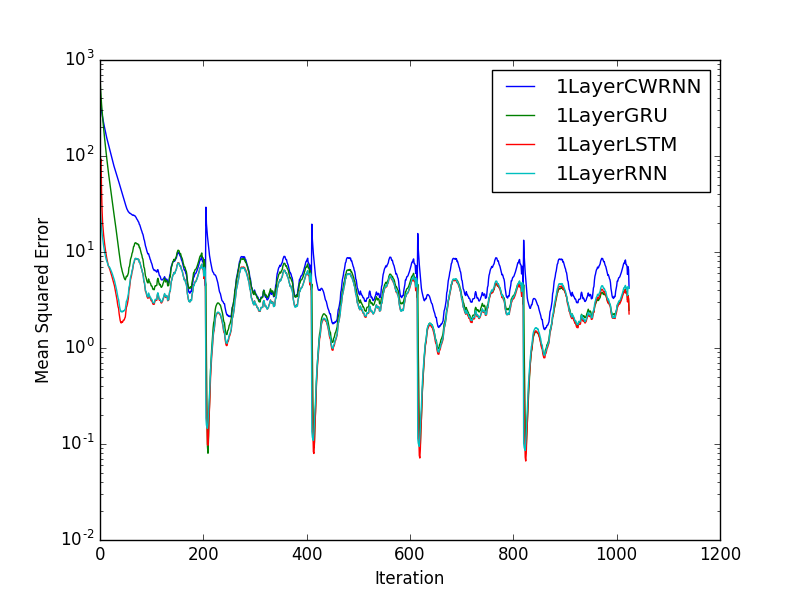
\includegraphics[width=0.8\textwidth]{1LayerComparison.png}
	\caption{Graph comparing error rates of various 1 layer recurrent networks
	during training}
	\label{fig:1layer}
\end{figure}

Based on figure~\ref{fig:1layer}, the collected data reveals that with one
layer, all the recurrent network types have similar errors. However, it should
be noted that the scale is logarithmic, and also that the models do not seem to
decrease their error significantly over the iterations suggesting that perhaps
the impelementation of the training of the models was incorrect. However, the
graph depicting the error rates of the 3 layered models is clearer.

\begin{figure}[H]
	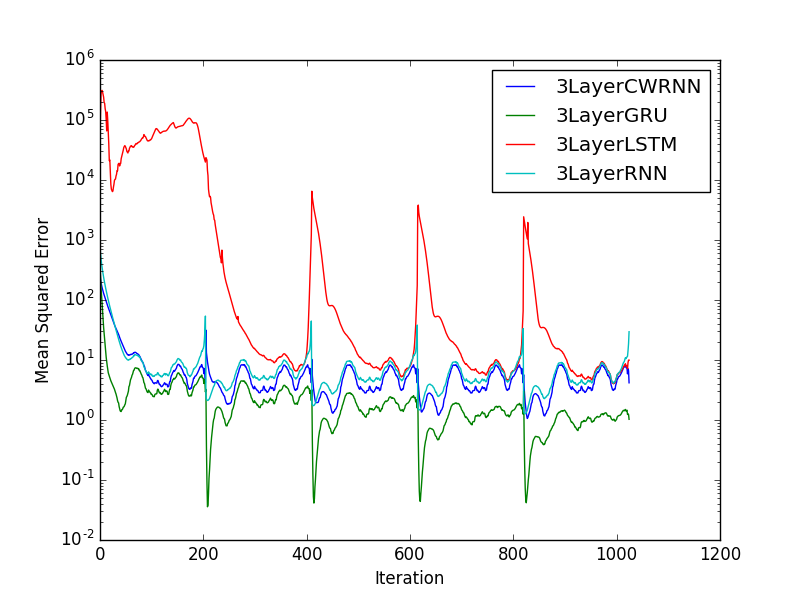
\includegraphics[width=0.8\textwidth]{3LayerComparison.png}
	\caption{Graph comparing error rates of various 3 layer recurrent networks
	during training}
	\label{fig:3layer}
\end{figure}

After considering figure~\ref{fig:3layer}, it becomes obvious that the model
requiring the least iterations to converge the quickest to a low error rate is
the 3 layer GRU, followed by the 3 layer clockwork recurrent network. The LSTM
error rate is significantly higher than the rest of the models, considering the
LSTM had comparable performance on the first graph, suggesting that
perhaps the model was implemented incorrectly.

\section{Observations}
Although the clockwork recurrent neural network was thought to be faster, it
seems that the GRU and LSTM outperformed it in terms of speed. Thus, it seems in
terms of time efficiency, the GRU is one of the faster one, with the standard
vanilla recurrent network being the fastest by far. The vanilla recurrent neural
network also had comparable errors to the other models, which makes it seem like
the best choice in terms of music generation.

The error of the LSTM seems to be the highest at all times, suggesting that
perhaps the LSTM takes significantly longer to train or that the LSTM simply
does not have as much modeling power as a simple vanilla recurrent network,
which is difficult to believe, simply due to how much more complex the LSTM
model is compared to the original recurrent network.

However, it should be noted that in these experiments, because of limits on
computational power and limits on time, the recurrent nets tested were fairly
small, so they did not generate anything that could be determined as music.
However, I went back and using these results, trained a larger, 4 layer GRU, and
was able to generate some audio that had a resemblence to some musical structure
within it, but it was essentially a direct copy of a section of the song that it
trained on.

\section{Conclusion}
Based on the benchmarks taken, it seems that in terms of speed, the vanilla
recurrent network is the fastest recurrent network for music generations.
However, in terms of the most accurate recurrent network model, the GRU is the
most effective, as demonstrated by the lower error rates that the GRU obtained
on the data in this experiment. However, as the error rates between all the
networks seemed similar, perhaps the most important factor in the training of a
recurrent network for music generation is speed, suggesting that perhaps the
vanilla recurrent network is the best network for training to generate music.

Some implications of these experiments are that in order for recurrent networks
to progress, the current method of training them must either be improved, or
a new architecture needs to be developed, since the nets did not decrease their
error rate to a low enough degress such that music could be heard, as my results
demonstrated. Thus, it seems that recurrent nets are still a ways away from the
task of music generation.

Furthermore, because the recurrent nets in this experiment were unable to
generate music, their ability to generate other sequences seem questionable as
well. Machine learning algorithms and technology may still need another couple
of years to develop before the idea of audio generation tasks in general become
possible, as music can be compared to other forms of audio as well, and perhaps
the primary algorithm for such audio generation will not be simple recurrent
nets, due to their difficulty to train and generate interesting sequences.

\newpage
\section{Appendix}
As the code is extremely lengthy, it is stored separately. To view the code,
refer to the online repository at: \url{https://github.com/Peachball/EE-DeepLearning}.

\newpage
\renewcommand{\refname}{Works Cited}
\begin{thebibliography}{9}
	\bibitem{theano}
		Bengio, Yoshua et al. \textit{Theano: A Python framework for fast
		computation of mathematical expressions.}.
		\url{http://deeplearning.net/software/theano}. Accessed 30 Aug. 2016.

	\bibitem{widendeep}
		Cheng, Heng-Tze. ``Wide and Deep Learning: Better Together with
		Tensorflow.'' \textit{Google Research Blog}, 29 June 2016.
		\url{https://research.googleblog.com/2016/06/wide-deep-learning-better-together-with.html}.
		Accessed 29 Aug. 2016

	\bibitem{gru}
		Chung, Gulcehre, Cho, and Bengio. ``Empirical Evaluation of Gated
		Recurrent Models on Sequence Modeling.'' \textit{arXiv}
		\url{https://arxiv.org/pdf/1412.3555v1.pdf}. Accessed 20 Aug. 2016.

	\bibitem{forgetgate}
		Gers, Schmidhuber, and Cummings. ``Learning to Forget: Continual
		Prediction with LSTM." \textit{ISDIA}, 1999 pag. 1-19.
		\url{https://pdfs.semanticscholar.org/1154/0131eae85b2e11d53df7f1360eeb6476e7f4.pdf}.
		Accessed 30 Aug. 2016.

	\bibitem{lstmpeep}
		Gers, Schraudolph, and Schmidhuber. ``Learning Precise Timing with LSTM
		Recurrent Networks.'' \textit{Journal of Machine Learning Research},
		2002, pag. 115-143.
		\url{http://www.jmlr.org/papers/volume3/gers02a/gers02a.pdf}. Accessed 3
		Sept. 2016.

	\bibitem{xavier}
		Glorot, Xavier and Bengio, Yoshua. ``Understanding the difficulty of
		training deep feedforward neural networks.'' \textit{Journal of Machine
		Learning Research}, Vol 9, 2010, pag. 249-256.
		\url{http://jmlr.org/proceedings/papers/v9/glorot10a/glorot10a.pdf}.
		Accessed 30 Aug. 2016.

	\bibitem{rmsprop}
		Hinton, Geoffrey. ``Neural Networks for Machine Learning.'' University
		of Toronto.
		\url{http://www.cs.toronto.edu/~tijmen/csc321/slides/lecture_slides_lec6.pdf}.
		Accessed 29 Aug. 2016.

	\bibitem{lstm}
		Horchreiter, Sepp and Schmidhuber, Jurgen. ``Long Short-Term Memory.''
		\textit{Technical University of Munich (1997)}: 1--32.
		\url{http://deeplearning.cs.cmu.edu/pdfs/Hochreiter97_lstm.pdf}.
		Accessed 10 May 2016.

	\bibitem{matplotlib}
		Hunter, J.D. ``Matplotlib: A 2D graphics environment.''
		\textit{Computing in Science \& Engineering}, vol 9, no. 3, 2007, pag.
		90-95. \url{http://matplotlib.org/}. Accessed 9 Oct.  2016.

	\bibitem{rnntrain}
		Jaeger, Herbert. ``A Tutorial on training recurrent neural networks,
		covering BPTT, RTRL, EKF, and the ``echo state network'' approach.''
		\textit{German National Research Center for Information Technology},
		2013.
		\url{http://minds.jacobs-university.de/sites/default/files/uploads/papers/ESNTutorialRev.pdf}.
		Accessed 10 Sept. 2016.

	\bibitem{lstmbias}
		Jozefowicz, Zaremba, and Sutskever. ``An Empirical Exploration of Neural
		Network Architectures.'' \textit{JMLR}, vol 37.
		\url{http://jmlr.org/proceedings/papers/v37/jozefowicz15.pdf}. Accessed
		4 Sept. 2016.

	\bibitem{cw-rnn}
		Koutnik, Jan et al. ``A Clockwork RNN.'' \textit{Dalle Molle Institute
		for Artificial Intelligence Research}: n\. pag.
		\url{https://arxiv.org/pdf/1402.3511.pdf}. Accessed 25 May 2016.

	\bibitem{dlppt}
		LeCun, Yann, Yoshua Bengio, and Geoffrey Hinton. "Deep learning." Nature
		521.7553 (2015): 436-444.
		\url{http://www.bioinfo.org.cn/~casp/temp/DeepLearning.pdf}. Accessed 9 Oct. 2016

	\bibitem{nielbook}
		Nielsen, Michael. ``Chapter 1: Using neural nets to recognize
		handwritten digits.'' \textit{Neural Networks and Deep Learning},
		\url{neuralnetworksanddeeplearning.com/chap1.html}. Accessed 10 Sept. 2016.

	\bibitem{nielgrad}
		Nielsen, Michael. ``Chapter 5: Why are deep neural networks so hard to
		train?'' \textit{Neural Networks and Deep Learning},
		\url{neuralnetworksanddeeplearning.com/chap5.html}. Accessed 10 Sept. 2016.

	\bibitem{ngcourse}
		Ng, Andrew. ``Classification.'' \textit{Machine Learning}, Coursera.
		\url{https://www.coursera.org/learn/machine-learning/lecture/wlPeP/classification}.
		Accessed 6 Jul. 2016.

	\bibitem{ngrepr}
		Ng, Andrew. ``Hypothesis Representation.'' \textit{Machine Learning}, Coursera.
		\url{https://www.coursera.org/learn/machine-learning/lecture/RJXfB/hypothesis-representation}.
		Accessed 6 Jul. 2016.

	\bibitem{wavenet}
		Oord, Aaron van den, et al. "WaveNet: A Generative Model for Raw Audio."
		\url{https://deepmind.com/blog/wavenet-generative-model-raw-audio/}.
		Accessed 29 Nov. 2016.

	\bibitem{syntaxnet}
		Petrov, Slav. ``Announcing SyntaxNet: The World's Most Accurate Parser
		Goes Open Source.'' \textit{Google Research Blob}, 12 May 2016.
		\url{https://research.googleblog.com/2016/05/announcing-syntaxnet-worlds-most.html}.
		Accessed 20 Aug. 2016.

	\bibitem{graddescent}
		Ruder, Sebestian. ``An Overview of Gradient Descent Algorithms.''
		\textit{Sebestian Ruder}, 19 Jan. 2016,
		\url{sebastianruder.com/optimizing-gradient-descent/index.html#gradientdescentvariants
		}. Accessed 10 Sept. 2016

	\bibitem{bptt}
		Werbos, Paul J. ``Backpropagation Through Time: What It Does and How to
		Do It.'' \textit{Proceedings of the IEEE}, vol. 78, no. 10, 1990,
		\url{deeplearning.cs.cmu.edu/pdfs/Werbos.backprop.pdf}. Accessed 11 Oct.
		2016.

\end{thebibliography}

%Cool sources that weren't mentioned in this paper
\begin{comment}
	\bibitem{convrnn}
		Abdel-Hamid, Deng, and Yu. ``Exploring Convolutional Neural Network
		Structures and Optimization Techniques for Speech Recognition.''
		\textit{Microsoft Research}, 2013, pag. 3366-3370. Web. 20 Aug. 2016.

	\bibitem{rprop}
		Riedmiller, Martin and Braun, Henrich. ``A Direct Adaptive Method for
		Faster Backpropagation Learning: The RPROP Algorithm.'' \textit{The
		University of Karlsruhe}, 1993, pag. 586-591. Web. 20 Aug. 2016.

	\bibitem{rbm}
		Hinton, Geoffrey. ``A Practical Guide to Training Restricted Boltzmann
		Machines.'' \textit{University of Toronto (2010)}: 1--20. Web. 10 May
		2016.

	\bibitem{rbm intro}
		Fischer, Asja and Igel, Christian. ``An Introduction to Restricted
		Boltzmann Machines. \textit{University of Copenhagen (2012)}: 14--36. Web.
		10 May 2016.

	\bibitem{deepnetworktrainers}
		Larochelle, Hugo et al. ``Exploring Strategies for Training Deep Neural
		Networks.'' \textit{Journal of Machine Learning Research} (2009): n\. pag.
		Web. 10 May 2016.

	\bibitem{dnn dimensionality}
		Hinton, G.E. and Salakhutdinov, R. R. ``Reducing the Dimensionality of
		Data with Neural Networks.'' \textit{Science} (2006). 504--507. Web. 10
		May 2016

	\bibitem{unsupervised}
		Erhan, Dumitru et al. ``Why Does Unsupervised Pre-training Help Deep
		Learning?'' \textit{University of Montreal}:201--208. Web. 10 May 2016.
\end{comment}

\end{document}
